\documentclass{VUMIFPSbakalaurinis}
\usepackage{algorithmicx}
\usepackage{algorithm}
\usepackage{algpseudocode}
\usepackage{amsfonts}
\usepackage{amsmath}
\usepackage{bm}
\usepackage{caption}
\usepackage{color}
\usepackage{float}
\usepackage{graphicx}
\usepackage{listings}
\usepackage{subfig}
\usepackage{wrapfig}
\usepackage[table,xcdraw]{xcolor}
\usepackage{enumitem}
\usepackage{longtable}
\setitemize{noitemsep,topsep=0pt,parsep=0pt,partopsep=0pt}
\setenumerate{noitemsep,topsep=0pt,parsep=0pt,partopsep=0pt}

\hbadness=100000
% Titulinio aprašas
\university{Vilniaus universitetas}
\faculty{Matematikos ir informatikos fakultetas}
\department{Programų sistemų studijų programa}
\papertype{Magistro baigiamasis darbas}
\title{Srautinio apdorojimo sistemų balansavimas taikant skatinamąjį mokymąsi}
\titleineng{Balancing stream processing systems using reinforcement learning}
\author{Vytautas Žilinas}
\supervisor{Andrius Adamonis}
\reviewer{Prof. dr. Aistis Raudys}
\date{Vilnius – \the\year}

% Nustatymai
% \setmainfont{Palemonas}   % Pakeisti teksto šriftą į Palemonas (turi būti įdiegtas sistemoje)
\bibliography{bibliografija}

\begin{document} 
\maketitle

\cleardoublepage\pagenumbering{arabic}
\setcounter{page}{2}

\sectionnonumnocontent{Santrauka}
TODO
\raktiniaizodziai{srautinis apdorojimas, skatinamasis mokymasis, balansavimas, "Heron", REINFORCE, DQN, ACER}   

\sectionnonumnocontent{Summary}
TODO
\keywords{stream processing, reinforcement learning, balancing, "Heron", REINFORCE, DQN, ACER}

\tableofcontents

\sectionnonum{Įvadas}

Realaus laiko duomenų apdorojimas (angl. real–time data processing) yra jau senai nagrinėjamas kaip vienas iš būdų apdoroti didelių kiekių duomenis (angl. Big data). Viena iš didelių duomenų apdorojimo tipinių architektūrų yra srautinis apdorojimas. Srautinis duomenų apdorojimas (angl. stream processing) – lygiagrečių programų kūrimo modelis, pasireiškiantis sintaksiškai sujungiant nuoseklius skaičiavimo komponentus srautais, kad kiekvienas komponentas galėtų skaičiuoti savarankiškai \cite{shortstreamproc}. 

Srautinio apdorojimo sistemoms valdyti yra naudojami srautinio apdorojimo varikliai. Yra keli pagrindiniai srautinio apdorojimo varikliai: „Apache Storm“, „Apache Spark“, „Heron“ ir kiti. „Apache Storm“ ir „Heron“ apdoroja duomenis duomenų srautais, o „Apache Spark“ mikro–paketais \cite{karau2015learning}. „Heron“ srautinio apdorojimo variklis, buvo išleistas „Twitter“ įmonės 2016 metais, kuris buvo sukurtas siekiant patobulinti įmonėje plačiai naudojama „Apache Storm“ srautinio apdorojimo variklį \cite{openSourcing}. Šiame darbe bus naudojamas „Heron“, kadangi jis yra naujesnis ir greitesnis srautinio apdorojimo variklis nei „Apache Storm“ \cite{twitterHeron}. 

Srautinio apdorojimo sistemų balansavimas (angl. auto–tuning) – tai sistemos konfigūracijos ir komponentų valdymas siekiant užtikrinti sistemos greitaveiką neprarandant stabilumo ir optimalaus resursų išnaudojimo. Kadangi srautinio apdorojimo sistemų komponentai yra kuriami kaip lygiagretus skaičiavimo elementai, jie gali būti plečiami horizontaliai ir vertikaliai \cite{shortstreamproc} keičiant sistemų konfigūraciją. Tačiau lygiagrečių elementų kiekio keitimas nėra vienintelis būdas optimizuoti resursų išnaudojimą. Kiekvienas variklis turi savo rinkinį konfigūruojamų elementų. Pavyzdžiui, darbe naudojamas „Heron“ variklis leidžia valdyti savo posistemes ir pateiktas srautinio apdorojimo sistemas naudojant 56 konfigūruojamus parametrus \cite{configDocument}.

Yra skirtingi būdai kaip gali būti parenkama tinkama konfigūracija. Kadangi srautinio apdorojimo sistemų apkrovos gali būti skirtingų pobūdžių (duomenų kiekis, skaičiavimų sudėtingumas, nereguliari apkrova), o inžinieriai kurdami ir konfigūruodami taikomąsias sistemas išbando tik kelis derinius ir pasirenka labiausiai tinkanti \cite{selfRegulatingStreaming}, lieka daug skirtingų nepatikrintų konfigūracijos variantų. Optimalios konfigūracijos suradimas yra NP sudėtingumo problema \cite{automateTuning}, kadangi žmonėms yra sunku suvokti didelį kiekį konfigūracijos variacijų. 
Vienas iš būdų automatiškai valdyti konfigūraciją buvo pasiūlytas 2017 metų straipsnyje „Dhalion: self–regulating stream processing in heron“, kuriame autoriai aprašo savo sukurtą sprendimą „Dhalion“, kuris konfigūruoja „Heron“ srautinio apdorojimo sistemas pagal esamą apkrovą ir turimus resursus, tai yra, jei apdorojimo elementų išnaudojimas išauga virš 100\%, „Dhalion“ padidina lygiagrečiai dirbančių apdorojimo elementų kiekį \cite{dhalion}. Tačiau toks sprendimas leidžia reguliuoti tik elementų lygiagretumą ir tai daro tik reaktyviai.

Vienas iš naujausių tyrimo krypčių nagrinėjančių srautinio apdorojimo sistemų balansavimą – mašininis mokymasis. Vienas iš tokių bandymų aprašytas 2018 metų straipsnyje „Auto–tuning Distributed Stream Processing Systems using Reinforcement Learning“\cite{vaquero2018autotuning} kuriame atliktas tyrimas – „Apache Spark“ sistemos balansavimui naudojamas skatinamojo mokymo REINFORCE algoritmas, kuris, pagal dabartinę konfigūraciją ir renkamas metrikas, keitė srautinio apdorojimo sistemos konfigūracijos parametrus. Šiame tyrime pasiūlytas sprendimas, naudojantis mašininį mokymąsi, suranda efektyvesne konfigūraciją per trumpesnį laiką nei žmonės, o tokiu būdu išskaičiuotą konfigūraciją naudojanti sistema pasiekia 60–70\% mažesnį vėlinimą, nei naudojanti ekspertų rankiniu būdu nustatytą konfigūraciją. \cite{vaquero2018autotuning}. 

Skatinamasis mokymasis yra vienas iš mašininio mokymosi tipų. Šis mokymasis skiriasi nuo kitų, nes tokio tipo tinklai mokosi darydami bandymus, klysdami ir pagal tai mokydamiesi. Vienas iš pagrindinių privalumų naudojant skatinamąjį mokymąsi balansavimui – nereikia turėti išankstinių duomenų apmokymui, kas leidžia jį paprasčiau pritaikyti skirtingoms srautinio apdorojimo sistemų apkrovoms. Tačiau tokio tipo mašininis mokymasis turi ir problemų: sudėtinga aprašyti tinkamos konfigūracijos atlygio (angl. reward) funkciją ir balansą tarp tyrinėjimo ir išnaudojimo tam, kad nebūtų patiriami nuostoliai \cite{selfRegulatingStreaming}.

Yra sukurta daug skatinamojo mokymosi algoritmų (Monte Carlo, Q–learning, Deep Q Network ir kiti), šiame darbe yra apžvelgti algoritmai, kuriuos naudojo kiti autoriai savo tyrimuose susijusiuose su srautinio apdorojimo sistemų veikimo gerinimu ir pasirinkti keli iš jų siekiant patikrinti ar skatinamasis mokymasis yra tinkamas srautinių sistemų balansavimui ir kuris skatinamojo mokymosi algoritmas pasiekia geriausius rezultatus su tam tikru kiekiu apmokymo žingsnių. Tyrimui naudojami REINFORCE, Deep Q network bei Actor–Critic with Experience Replay skatinamojo mokymosi algoritmai ir tiriama kaip kiekvienas iš jų pasirodo su vienodu kiekiu apmokymo žingsnių ir tokia pačia srautinio apdorojimo sistema.

Tikslas: Ištirti skatinamojo mokymosi tinkamumą srautinio apdorojimo sistemų balansavimui. 

Uždaviniai:

\begin{enumerate}
    \item Sudaryti srautinio apdorojimo sistemų balansavimo modelį ir nustatyti valdymo metrikas ir jų siekiamas reikšmes, kurios bus naudojamos eksperimentinėje sistemoje.
    \item Parinkti srautinę apdorojimo sistemą ir skatinamojo mokymosi algoritmus eksperimentui, atsirenkant iš algoritmų ir sistemų, aprašomų literatūroje.
    \item Sukurti eksperimentinį sprendimą su pasirinkta srautinio apdorojimo sistema ir atlikti eksperimentus su skirtingais skatinamojo mokymosi algoritmais.
    \item * Gal šito iš vis nereikia *  Palyginti eksperimento rezultatus su alternatyvomis – „Heron“ su standartine konfigūracija  * ar reikia –> * bei „Heron“ balansavimas rankiniu būdu. 
\end{enumerate}



\section{Srautinio apdorojimo sistemų matavimas ir derinimas}
\subsection{Srautinio apdorojimo sistemos}
Srautinis duomenų apdorojimas (angl. stream processing) – terminas naudojamas apibrėžti sistemas sudarytas iš skaičiavimo elementų (angl. modules) galinčių skaičiuoti lygiagrečiai ir kurios bendrauja kanalais. Tokių sistemų elementai dažniausiai skirstomi į tris klases: šaltinius (angl. sources), kurie paduoda duomenis į sistemą, filtrus (angl. filters), kurie atlieka tam tikrus vienetinius (angl. atomic) skaičiavimus ir nuotakus (angl. sink), kurie perduoda duomenis iš sistemų \cite{stephens1997survey}. 
\begin{figure}[H]
    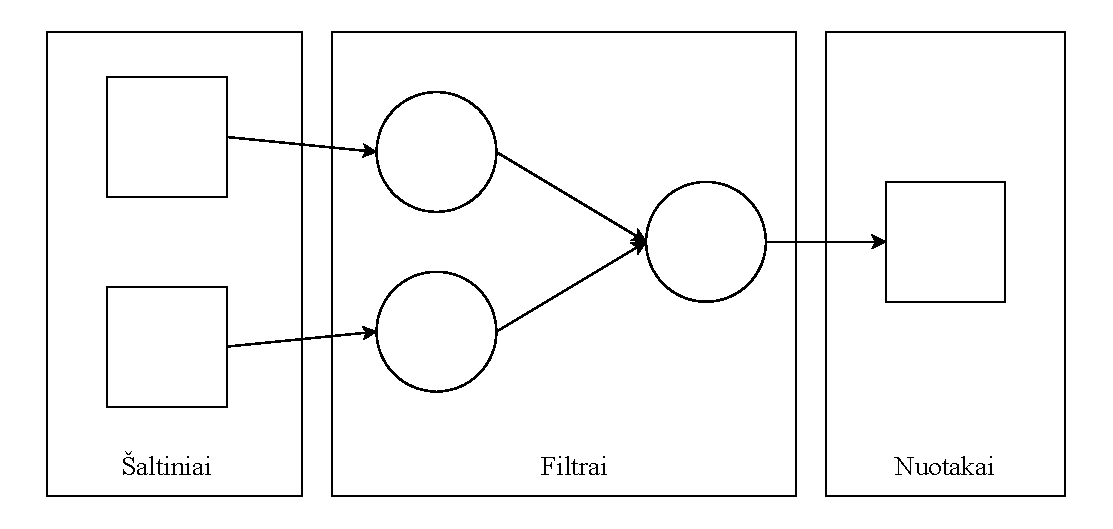
\includegraphics[width=15cm]{img/Srautinio apdorojimo sistema.pdf}
    \caption{Srautinio apdorojimo sistemos pavyzdys}
    \label{srautinio–apdorojimo–sistema}
\end{figure} 
Srautinio apdorojimo sistemos literatūroje yra vaizduojamos orientuotais grafikais (\ref{srautinio–apdorojimo–sistema} pav.). Srautinio apdorojimo sistemos skiriasi nuo reliacinio modelio šiais aspektais \cite{babcock2002models}: 
\begin{itemize}
    \item Duomenys į sistemą patenka tinklu, o ne iš fizinių talpyklų.
    \item Duomenų patekimo tvarka negali būti kontroliuojama.
    \item Duomenų kiekis yra neapibrėžtas.
    \item Duomenys apdoroti srautinio apdorojimo sistema yra pašalinami arba archyvuojami, t.y. juos pasiekti po apdorojimo yra sunku. 
\end{itemize}
\subsubsection{Duomenų vykdymas}
Srautinio apdorojimo sistemų veikimui reikalingas srautinio apdorojimo variklis (angl. stream processing engine). Šie varikliai yra skirti srautinio apdorojimo sistemų vykdymui, dislokavimui, plečiamumo (angl. scaling) užtikrinimui ir gedimų tolerancijai (angl. fault–tolerance) \cite{zhao2017taxonomy}. Populiariųjų srautinio apdorojimo variklių pavyzdžiai: „Apache Storm“, „Apache Heron“, „Apache Spark“, „Apache Samza“ ir t.t \cite{roger2019comprehensive}. 
Duomenų vykdymas gali būti išskaidytas į tris elementus \cite{zhao2017taxonomy}: 
\begin{itemize}
    \item Planavimas (angl. scheduling) – duomenų apdorojimo užduočių planavimas, kuris daro įtaką bendram srautinio apdorojimo sistemos veikimui \cite{falt2011task}. Pavyzdžiui, „Apache Samza“ naudoja „Apache YARN“ resursų valdymo sistemos planavimo posistemę, kuri skirsto resursus \cite{noghabi2017samza} 
    \item Plečiamumas (angl. scalability) – daug apdorojimo branduolių turinčios sistemos turi gebėti apdoroti didėjanti kiekį užduočių ir galimybę išskirti resursus sistemai, kad ji galėtų susidoroti su didėjančiu kiekiu duomenų \cite{bondi2000characteristics}. Srautinio apdorojimo varikliai turi užtikrinti srautinio apdorojimo sistemų plečiamumą \cite{stonebraker20058}.    
    \item Išskirstytas skaičiavimas (angl. distributed computation) – tarpusavyje nesusiję skaičiavimo elementai turi naudotojui atrodyti kaip viena darni sistemą \cite{tanenbaum2007distributed}. Srautinio apdorojimo varikliai turi užtikrinti darbų paskirstymą ir skaičiavimo įrenginių koordinaciją, kad kuo daugiau duomenų būtų apdorojami vienu metu \cite{zhao2017taxonomy}.
\end{itemize}
Srautinio apdorojimo sistemos turi viena pagrindinį elementą – srauto procesorių (angl. stream processor), kuris apibrėžia sistemos elementus, aprašo kaip šie sistemos elementai sujungti ir pateikia nustatymus elementams \cite{zhao2017taxonomy}. Pavyzdžiui, „Apache Storm“ ir „Heron“ šis elementas vadinimas „topology“, kuris yra užrašomas Java kalba, naudojant „Apache Storm“ pateiktą biblioteką \cite{iqbal2015big}.
\subsubsection{Duomenų priėmimas}
Į srautinio apdorojimo sistemą duomenys patenka per šaltinius, kurie šiuos duomenis perduoda tolimesniems elementams. Dažniausiai duomenis perduodami į sistemą naudojant žinučių eiles (angl. message queues), nes jos turi buferi, kuris leidžia mažinti greičių skirtumus tarp duomenų gavimo ir duomenų apdorojimo ir žinučių eilių brokeriai gali išfiltruoti duomenis ir nukreipti juos į tinkamus šaltinius \cite{kamburugamuve2016survey}. Tačiau šaltiniai turi turėti galimybę rinkti išsaugotus duomenis ir priimti ateinančius naujus duomenis \cite{stonebraker20058}, todėl, nors ir šaltiniai dažniausiai skirti priimti srautinius duomenis, jie turi taip pat gebėti naudoti duomenis iš talpyklų \cite{zhao2017taxonomy}. 

\subsection{Srautinio apdorojimo sistemų matavimas}
Svarbiausias srautinio apdorojimo sistemų reikalavimas – duomenų apdorojimas ir rezultatų grąžinimas negali turėti atsilikimo – didelių apimčių srautiniai duomenys turi būti apdorojami taip pat greitai kaip jie patenka į sistemą \cite{stonebraker20058}. Tam, kad galima būtų užtikrinti šį reikalavimą, turi būti renkamos srautinio apdorojimo sistemų metrikos ir matuojama bendra greitaveiką.

\subsubsection{Srautinio apdorojimo sistemų metrikos}
Pagrindinės kitų autorių naudojamos metrikos srautinio apdorojimo sistemų matavimui:
\begin{itemize}
    \item Pralaidumas (angl. Throughput) – per tam tikrą laiko tarpą apdorojamų įvykių kiekis.
    \item Vėlinimas (angl. Latency) – laiko intervalas nuo apdorojimo arba įvykio pradžios iki apdorojimo pabaigos.
\end{itemize}
Vėlinimas ir pralaidumas dažniausiai nepriklauso vienas nuo kito – sistemos, apdorojančios srautus mikro–paketais, turi didesnį pralaidumą, tačiau atsiranda papildomas vėlinimas, kol laukiama duomenų paketo apdorojimo pradžios \cite{Karimov2018BenchmarkingDS}. \par

\cite{stonebraker20058} straipsnyje minima, jog srautinio apdorojimo sistemos naudotojas turi išbandyti savo sistemą su tiksliniu darbo krūviu ir išmatuoti jos pralaidumą ir vėlinimą prieš naudodamas ją realiomis sąlygomis. \cite{Karimov2018BenchmarkingDS} lygina srautinio apdorojimo variklius ir matavimui naudoja vėlinimą, kurį išskaido į įvykio vėlinimą (angl. event–time latency) – laiko intervalas nuo įvykio laiko iki rezultato gavimo iš srautinio apdorojimo sistemos ir apdorojimo vėlinimą (angl. processing–time latency) – laiko intervalas nuo duomens patekimo į srautinio apdorojimo sistemą iki rezultato grąžinimo. Autoriai atlieka šį skaidymą, nes sistemų vertinime dažnai ignoruojamas įvykio laikas ir rezultatuose gaunamas daug mažesnis vėlinimas, nei tikras. Taip pat autoriai išskiria darnų pralaidumą (angl. sustainable throughput) – didžiausią apkrovą įvykių, kurią sistema gali apdoroti be pastoviai augančio įvykių vėlinimo, todėl savo eksperimentuose autoriai užtikrina, kad duomenų generavimo greitis atitiktų sistemos darnų pralaidumą. Kad sužinoti darnų pralaidumą, sistemos autoriai pradžioje leidžia labai didelį srautą duomenų ir mažina jį kol sistemos apdorojimas susivienodina su generavimo greičiais. Visus vėlinimo rezultatus autoriai pateikia maksimalaus pralaidumo apdorojimo ir 90\% pralaidumo apdorojimo vidurkiais, minimumais, maksimumais ir kvantiliais (90, 95, 99). \cite{hirzel2014catalog} autoriai nagrinėja srautiniam apdorojimui galimas optimizacijas ir matavimui naudoja normalizuotą pralaidumą (naudojamas vienetas kaip vidurkis), kadangi tai leidžia lengviau palyginti santykinę greitaveiką. Taip pat, \cite{hirzel2014catalog} pastebi, nors ir yra daug metrikų, kuriomis galima matuoti optimizacijos efektus: pralaidumas, vėlinimas, paslaugos kokybė (angl. quality of service), energijos ir tinklo panaudojimas, tačiau dažniausiai pagerinus pralaidumą pagerėja ir visos kitos metrikos. \cite{Qian2016Benchmarking} srautinių apdorojimo sistemų matavimui naudoja pralaidumą (skaičiuojama baitais per sekundę) ir vėlinimą, kaip vidurkį nuo duomens patekimo į sistemą iki apdorojimo pabaigos. Taip pat, kadangi autoriai lyginą srautinio apdorojimo variklius, jie įveda metriką gedimų toleravimo (angl. fault tolerance) matavimui – išjungiamas tam tikras kiekis elementų ir matuojamas pralaidumas ir vėlinimas. \cite{zhang2020heron} palyginimui naudoja sistemos įvykdymo vėlinimą (angl. system completion latency), kuris rodo vidutinį laiko tarpą per kurį duomuo nukeliauja nuo šaltinio iki sistemos galutinio taško. Šio straipsnio autoriai skaičiavo vidutinį laiką 5 sekundžių intervalais. Taip pat \cite{zhang2020heron} matavimui naudoja kiekvienos instancijos (angl. instance) CPU apkrovą, kiekvieno darbinio mazgo (angl. worker node) CPU apkrovą ir apkrovą tarp instancijų/mazgų, kadangi \cite{zhang2020heron} užduotis – patobulinti esamą planavimo posistemę. \cite{dhalion} matavimui naudoja pralaidumą per minutę. \cite{vaquero2018autotuning} tyria labai panašią problemą – srautinių apdorojimo sistemų balansavimą taikant skatinamąjį mokymą ir matavimui naudoja vėlinimo 99 percentilę. \cite{Chintapalli2016Benchmarking} srautinio apdorojimo variklių vertinimo tyrimui naudoja vėlinimą.

\begin{longtable}{|p{0.2\linewidth}|p{0.2\linewidth}|p{0.2\linewidth}|}
    \caption{Metrikos naudojamos tiriant srautinio apdorojimo sistemų greitaveiką}
    \label{metrikos}\\
    \hline
    \rowcolor[HTML]{C0C0C0} 
    Šaltinis                 & Vėlinimas                        & Pralaidumas                    \\ \hline
    \cite{stonebraker20058}  & Taip                             & Taip                           \\ \hline
    \cite{Karimov2018BenchmarkingDS} & Taip                     & Taip                           \\ \hline
    \cite{hirzel2014catalog} & Ne                               & Taip                           \\ \hline
    \cite{Qian2016Benchmarking} & Taip                          & Taip                           \\ \hline
    \cite{zhang2020heron}    & Taip                             & Ne                             \\ \hline
    \cite{dhalion}           & Ne                               & Taip                           \\ \hline
    \cite{vaquero2018autotuning} & Taip                         & Ne                             \\ \hline
    \cite{Chintapalli2016Benchmarking} & Taip                   & Ne                             \\ \hline
\end{longtable}

Pagal literatūros analizę (\ref{metrikos} len.) matoma, kad dauguma autorių renkasi vertinti tik pagal vieną metriką ir dažniau matavimui naudojamas vėlinimas. Taip pat \cite{vaquero2018autotuning}, naudojantis skatinamąjį mokymą, matavimui naudoja vėlinimą ir \cite{Chintapalli2016Benchmarking} straipsnis, kuris siūlo srautinio apdorojimo sistemų vertinimo sprendimą, naudoja vėlinimą. 

\subsubsection{Srautinio apdorojimo sistemos pobūdis}

Srautinio apdorojimo sistemos gali turėti skirtingą elementų išsidėstymą ir nuo to priklausys jų greitaveiką. \cite{Karimov2018BenchmarkingDS} matavimui naudoja du filtrus – agregavimo, kuris skaičiuoja visus pirkimus ir jungimo (angl. join), kuris skaičiuoja duomenis pagal tam tikrą bendrą rodiklį iš abiejų duomenų srautų. \cite{Qian2016Benchmarking} srautinio apdorojimo variklių palyginimui naudoja septynis skirtingus uždavinius. Vienas iš jų yra WordCount uždavinys, kuris yra plačiai priimtas kaip didelių duomenų apdorojimo sistemos matavimo standartas \cite{huang2010hibench}. Šis uždavinys susidaro iš dviejų filtrų: pirmas išskaido teksto eilutę į žodžius, o antras agreguoja kiekvieno žodžio bendrą skaitiklį ir atnaujina bendrą žodžių panaudojimo dažnio rezultatą, kuriame raktas – žodis, o reikšmė skaičius, kuris rodo kiek kartojosi šis žodis (\ref{wordcount} pav.). 
\begin{figure}[H]
    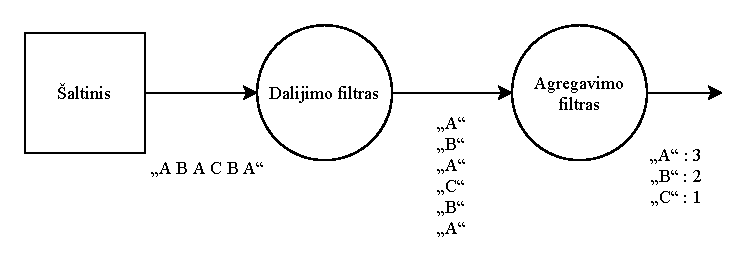
\includegraphics[width=15cm]{img/wordcount.pdf}
    \caption{WordCount sistemos pavyzdys}
    \label{wordcount}
\end{figure} 
\cite{zhang2020heron} autoriai naudoja SentenceWordCount sistemą, kuri yra identiška \ref{wordcount} paveikslėlyje pavaizduotai sistemai. Bei autoriai sukūrė FileWordCount sistemą, kuri atlieka tą patį kaip ir SentenceWordCount, tačiau šaltinis negeneruoja žodžius, o skaito iš tekstinio dokumento ir taip pat naudoja egzistuojančią Yahoo srautinio apdorojimo vertinimą (angl. benchmarking) \cite{Chintapalli2016Benchmarking}. \cite{dhalion} autoriai naudoja WordCount eksperimentui. \cite{vaquero2018autotuning} eksperimentams naudoja Yahoo srautinio apdorojimo variklių vertinimą \cite{Chintapalli2016Benchmarking} ir taip pat atlieka bandymus su realiais daiktų interneto (angl. internet of things) įmonės duomenimis. \cite{Chintapalli2016Benchmarking} pateikia srautinio apdorojimo sistemą skirtingu srautinio apdorojimo variklių vertinimui. Ši sistema analizuoja reklamas pagal kampaniją ir matomumą ir rezultatus deda į Redis duomenų bazę. Ši sistema sukurta taip, kad aprėptų visas srautinio apdorojimo sistemos savybes (\ref{yahoo} pav.).
\begin{figure}[H]
    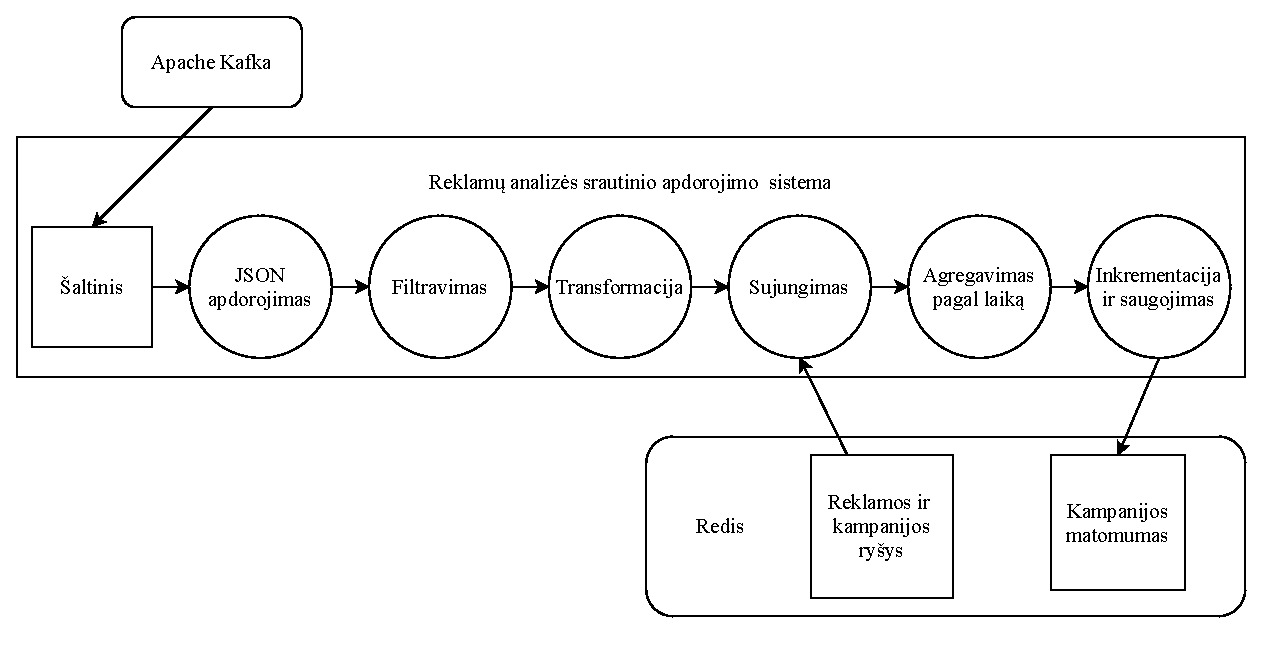
\includegraphics[width=15cm]{img/yahoo.pdf}
    \caption{Reklamų analizės sistema \cite{Chintapalli2016Benchmarking}}
    \label{yahoo}
\end{figure} 

Straipsniai (\cite{Qian2016Benchmarking, huang2010hibench, dhalion}) naudoja WordCount (\ref{wordcount} pav.), o \cite{Chintapalli2016Benchmarking, vaquero2018autotuning} naudoja Reklamų analizės srautinę apdorojimo sistemą (\ref{yahoo} pav.). Reklamų analizės srautinio apdorojimo sistemos privalumas palyginus su WordCount srautinio apdorojimo sistema - galimybė valdyti į sistemą patenkančių duomenų srautą, kas leidžia atlikus tyrimą teigti, jog duomenų apdorojimo pastovumas nedarė įtakos rezultatams.

\subsubsection{Srautinio apdorojimo sistemų matavimo duomenys}

Vertinant sistemų greitaveiką reikia atsižvelgti ir į testavimui naudojamus duomenis. \cite{Karimov2018BenchmarkingDS} naudoja žaidimų kūrimo įmonės Rovio duomenis ir naudoja du duomenų srautus – pirkimo srautas, kuriame siunčiami kortežai (angl. tuples) sudaryti iš nupirktos valiutos kiekio, laiko ir naudotojo, kuris ją nupirko ir reklamų srautas, kuris siunčia valiutos reklamas tam tikru laiku. Šiame sprendime duomenis generuojami naudojant normalizuotą paskirstymą ant raktinio lauko. \cite{Qian2016Benchmarking} naudoja tekstinius duomenis iš AOL paieškos variklio ir apdoroja juos pagal pasirinktus uždavinius. \cite{zhang2020heron} matavimui naudoja šaltinių generuojamą tekstą, kadangi lyginamas tas pats srautinio apdorojimo variklis tik su patobulinta planavimo posisteme ir naudoja iš anksto sugeneruotą tekstą patalpintą į tekstinį dokumentą. \cite{Chintapalli2016Benchmarking} aprašo sistemą, kuri daro skirtingų srautinio apdorojimo variklių vertinimą. Šiam vertinimui naudojami duomenys simuliuojantys reklamas ir reklamų kampanijas ir todėl autoriai naudoja savo sukurtą duomenų generatorių. 

\subsection{Srautinio apdorojimo sistemų derinimas}
Sistemų greitaveika yra tiesiogiai susijusi su konfigūravimo parametrais, kurie valdo tokius aspektus kaip: atminties valdymas, gijų skaičius, planavimas, resursų valdymas \cite{lu2019speedup}. Taip pat, neteisingi nustatymai turi nuostolingus efektus sistemos greitaveikai ir stabilumui \cite{herodotou2011starfish}. 

\cite{herodotou2020survey} išskiria 3 pagrindinius automatinio derinimo iššūkius:
\begin{enumerate}
    \item Didelė ir sudėtinga parametrų erdvė – „Apache Spark“ ir „Apache Storm“ turi virš 150 konfigūruojamų parametrų \cite{Bilal2017Towards, petridis2016spark}. Taip pat, nustatymų reikšmės, kurios tinka vienam uždaviniui, gali turėti neigiamos įtakos kitam \cite{herodotou2011starfish, Pooyan2016Uncertainty}.
    \item Sistemų mastas ir sudėtingumas – Sistemų administratoriai turi gebėti konfigūruoti didelius kiekius skaičiavimo mazgų, kurie gali turėti skirtingus CPU, atminties, tinklo tipus \cite{herodotou2020survey}.
    \item Pradinių duomenų statistikos trūkumas – įvedimo duomenys srautinėse apdorojimo sistemose yra realus srautai, kurie stipriai varijuoja savo apimtimi \cite{Dayarathna2018Recent}.
\end{enumerate}  

\cite{Trotter2017Into} nagrinėjantis tinkamos konfigūracijos radimą naudojant genetinius algoritmus „Apache Storm“ srautinio apdorojimo sistemoms nustatė, jog lygiagretumo laipsnis labiausiai daro įtaką srautinio apdorojimo sistemų greitaveikai. „Apache Heron“ srautinio apdorojimo variklis, kuris yra „Apache Storm“ su patobulinimais \cite{twitterHeron}, pateikia naują būdą kontroliuoti srautą – priešslėgis (angl. backpressure), kuris leidžia filtrui sulėtinti prieš jį einantį elementą, kas leidžia sumažinti vėlinimą ir taip pat gali būti naudojamas kaip greitaveikos praradimo indikatorius \cite{bansal2018trevor}.
Taip pat \cite{bansal2018trevor} nagrinėja „Apache Heron“ automatinį konfigūravimą naudojant iš anksto aprašytas taisykles. 

\section{Skatinamasis mokymasis}

PARAŠYTI ČIA APIE TAI KAD SKATINAMASIS YRA DALIS MAŠININIO
\subsection{Mašininis mokymasis srautinio apdorojimo sistemų derinimui}

\cite{herodotou2020survey} aprašo skirtingus sprendimus automatiniam konfigūravimui ir išskiria šiuos mašininio mokymosi privalumus:
\begin{itemize}
    \item Nebūtina suprasti sistemos, užduočių ir duomenų, kadangi naudojamas juodos dėžės (angl. black–box) principas.
    \item Mašininio mokymosi modelis pats save tobulina, ir yra vis tikslesnis kuo daugiau gauna duomenų. 
\end{itemize}
Šio straipsnio autoriai išskiria mašininio mokymosi iššūkius: 
\begin{itemize}
    \item Parametrų parinkimas – kadangi konfigūruojamų parametrų kiekis yra didelis \cite{Bilal2017Towards, petridis2016spark} ne visi iš jų vienodai daro įtaką greitaveikai, todėl pirma verta išsirinkti aktualiausius parametrus resursų valdymo, užduočių planavimo ir duomenų valdymo užduotims. Tam dažnai naudojama eksperto pagalba \cite{wang2016novel}, gidai arba eksperimentavimas. Tačiau galima naudoti mašininio mokymosi algoritmą koreliacijos nustatymui tarp parametrų ir greitaveikos \cite{vaquero2018autotuning, yang2012statistics}
    \item Mašininio mokymosi modelio pasirinkimas – kadangi yra nemažai skirtingų mašininio mokymosi metodų kurie tinka derinimo uždaviniui.
\end{itemize} 
Taip pat autoriai pateikia paketinio ir srautinio apdorojimo derinimą naudojant mašininį mokymąsi straipsnius (\ref{ml–in–stream} lentelėje pateikiami tik išrinkti srautinio apdorojimo pavyzdžiai).

\begin{longtable}{|p{0.3\linewidth}|p{0.35\linewidth}|p{0.25\linewidth}|}
    \caption{Srautinių sistemų derinimo naudojant mašininį mokymąsi pavyzdžiai \cite{herodotou2020survey}}
    \label{ml–in–stream} \\
    \hline
    \rowcolor[HTML]{C0C0C0} 
    Šaltinis                                        & Įvesties savybės                                                                    & Mašininio mokymosi metodai                 \\ \hline
    Zacheilas et al. \cite{zacheilas2015elastic}    & Rinkinys kelių konfigūracijos parametrų                                             & Gaussian Processes                         \\ \hline
    Li et al. \cite{li2016performance}              & Atminties dydžiai ir branduolių ir gijų kiekis skirtingose stadijose                & Support Vector Regression                  \\ \hline
    Trotter et al. \cite{Trotter2017Into}           & Darbinių procesų kiekis, vykdytojų kiekis                                           & Genetic Algorithm, Bayesian Optimization   \\ \hline
    Trotter et al. \cite{trotter2019forecasting}    & Vykdytojai, šaltinių ir filtrų lygiagretumas, acker lygiagretumas                   & Genetic Algorithm, Support Vector Machines \\ \hline
    OrientStream \cite{wang2017automating}          & Įvairios duomenų, plano, filtrų ir klasterio lygio savybės                          & Ensemble/ Incremental ML                    \\ \hline
    Vaquero et al. \cite{vaquero2018autotuning}     & Parametrai ir metrikos parinkti faktorinės analizės (angl. factor analysis) pagalba & Reinforcement Learning                     \\ \hline
\end{longtable}

\subsection{Skatinamasis mašininis mokymasis}
Standartiniame skatinamojo mašininio mokymosi algoritme agentas (angl. agent) yra prijungtas prie aplinkos (angl. environment) per stebėjimus (angl. perception) ir veiksmus (angl. action). Kiekvieną žingsnį agentas atlieka veiksmą ir to veiksmo vertė yra perduodama agentui per atlygį. Agentas renkasi veiksmus, kurie per laiko tarpą didina veiksmo atlygį. Tai pasiekiamą per tam tikrą laiko tarpą atliekant bandymus ir klystant, su papildoma algoritmų pagalba siekiant padidinti spėjimo efektyvumą ir sprendimų stabilumą \cite{reinf}.     

\subsubsection{Skatinamasis mokymasis srautinio apdorojimo sistemų veikimo gerinimui}

\cite{vaquero2018autotuning} nagrinėja srautinių sistemų derinimą naudojant skatinamąjį mokymąsi. Autoriai pradžioje naudoja Lasso path analysis algoritmą, kurio pagalba atlieka parametrų atranka, kad išrinktų svarbiausius parametrus pasirinktos metrikos valdymui. Konfigūracijos valdymui pasirinktas modifikuotas REINFORCE algoritmas. Atliktas eksperimentas su „Apache Spark“ ir pasiektas 60–70\% sumažintas vėlinimas.

\cite{ni2019generalizable} nagrinėja resursų valdymo problemą srautinio apdorojimo sistemose ir siūlo sprendimą naudojanti skatinamąjį mokymą, kuris daro optimizacijas pagal srautinės apdorojimo sistemos grafus. Eksperimentas atliekamas naudojant REINFORCE \cite{williams1992simple} algoritmą su Adam optimizacijos funkcija \cite{kingma2014adam} ir atliekamas eksperimentas naudojant tyrimui parašytą srautinio apdorojimo variklį ir sistemas. 

\cite{Li2018Model} nagrinėja planavimo problemos (apkrovos paskirstymas darbiniams elementams) sprendimą naudojant skatinamąjį mokymąsi. Autoriai siūlo naudoti Actor−Critic \cite{lillicrap2015continuous} metodą naudojant Deep Q Learning \cite{mnih2015human} tinklą kaip Actor ir bet kokį gilųjį neuroninį tinklą kaip Critic. Autorių rezultatai rodo 45\% greitaveikos padidėjimą lyginant su integruota „Apache Storm“ planavimo posisteme. 

\cite{Russo2019Reinforcement} nagrinėja srautinių sistemų dislokavimą naudojant skatinamąjį mokymą. Sprendžiama dislokavimo valdymo problema su skirtingais skaičiavimo mazgų tipais. Naudojamas Q Learning algoritmas su įvairiomis modifikacijomis (kombinuojama su tiksliais modeliais). Autoriai matuoja dislokavimo tikslumą ir konvergavimo greitį. 

\begin{longtable}{|p{0.3\linewidth}|p{0.6\linewidth}|}
    \caption{Skatinamojo mokymosi naudojimas}
    \label{ml–usage}\\
    \hline
    \rowcolor[HTML]{C0C0C0} 
    Šaltinis                         & Skatinamojo mokymosi algoritmas    \\ \hline
    \cite{vaquero2018autotuning}     & Adaptuotas REINFORCE \cite{williams1992simple}        \\ \hline
    \cite{ni2019generalizable}       & REINFORCE \cite{williams1992simple}  su Adam optimizacijos funkcija \cite{kingma2014adam}     \\ \hline
    \cite{Li2018Model}               & Deep Q Learning \cite{mnih2015human} ir Actor−Critic \cite{lillicrap2015continuous} \\ \hline
    \cite{Russo2019Reinforcement}    & Q–learning \cite{mnih2015human} su papildomomis funkcijomis \\ \hline
\end{longtable}

\subsubsection{Balansavimas naudojant REINFORCE algoritmą}
Straipsnis \cite{vaquero2018autotuning} nagrinėja automatinį balansavimą srautinio apdorojimo sistemų Apache Spark platformoje. Straipsnyje nagrinėjamas sprendimas susidaro iš trijų sistemų:
\begin{enumerate}
    \item Sistema, kurioje iš anksto sugeneruoti konfigūracijų deriniai leidžiami srautinio apdorojimo sistemose ir surenkamos metrikos bei konfigūracijos įverčiai. Gauti duomenis analizuojami naudojant Factor Analysis + k–means ir gaunamas sąrašas pagrindinių metrikų bei konfigūracijos elementai darantys daugiausiai įtakos greitaveikai. Ši sistema naudojama vieną kartą prieš leidžiant sekančią sistemą. 
    \item Sistema, kurioje surinktos metrikos ir konfigūracijos elementai yra leidžiami iš naujo ir naudojant Lasso path analizę konfigūracijos elementų sąrašas surūšiuojamas pagal įtaką greitaveikai. Tai daroma siekiant statistiškai užtikrinti, jog pasirinkti konfigūracijos elementai yra įtakingiausi. Ši sistema naudojama vieną kartą prieš leidžiant skatinamąjį mokymąsi.
    \item Pagrindinė mašininio mokymosi sistema, naudojanti REINFORCE algoritmą, kuri naudodamas surikiuotų konfigūracijos elementų sąrašą ir pagrindinių metrikų sąrašą periodiškai atnaujina konfigūraciją. Ši sistema paleidžiama tuo pačiu metu kaip ir srautinio apdorojimo sistema ir veikia visą laiką iki tyrimo pabaigos.
\end{enumerate}  
Eksperimentinis sprendimas buvo sukonfigūruotas kas 5 minutes atnaujinti vieną konfigūracijos elementą. Autoriams pavyko pasiekti 70\% sumažinta vėlinimą po 50 minučių, o veiksmų vertingumas pilnai konvergavo po 11 valandų.

\subsubsection{Deep Q Network algoritmas}
Deep Q Network yra Q Learning įgyvendinimas naudojant giliuosius neuroninius tinklus. Q Learning – skatinamojo mokymosi algoritmas, kuris bet kokiam baigtiniam Markovo pasirinkimo procesui randa optimalius sprendimus maksimizuojančius galutinio rezultato gavimą per bet kokį kiekį žingsnių pradedant nuo esamos būsenos \cite{melo2001convergence}. 
Q Learning naudoja Q funkciją, kurios įeigą yra būsenos ir veiksmo kombinacija, o rezultatas yra atlygio aproksimacija. Pradžioje visos Q reikšmės yra 0 ir algoritmas atlikdamas veiksmus pildo lentelę atnaujintomis reikšmėmis. Tačiau, kai veiksmų ir būsenų pasidaro per daug Q Learning algoritmo nebeužtenka ir tenka naudoti giliuosius neuroninius tinklus.  

Deep Q Network skiriasi nuo Q Learning tuo, kad vietoj būsenos ir veiksmų į jį paduodama būseną ir jis gražina Q reikšmę visų įmanomų veiksmų. Taip pat Deep Q Network naudoja patirties pakartojimą (angl. experience replay) – vietoj to, kad kurti sprendimą pagal paskutinį veiksmą yra paduodamas rinkinys atsitiktinių veiksmų pagal kurį algoritmas gali efektyviau mokytis. 

Deep Q Network algoritmo veikimas\cite{handson}:
\begin{enumerate}
    \item Perduoti aplinkos būseną į Deep Q Network, kuris gražins visus įmanomus veiksmus būsenai.
    \item Pasirinkti veiksmą naudojant \(\epsilon\)–greedy strategiją, kuriuo metu pasirenkamas atsitiktinis veiksmas arba pasirenkamas veiksmas turintis didžiausia Q reikšmę.
    \item Įvykdomas veiksmas ir pereinama į naują būseną. Šis perėjimas išsaugomas kaip patirties pakartojimo kortežas susidarantis iš būsenos, veiksmo, atlygio ir naujos būsenos.
    \item Pasirenkamas atsitiktinis rinkinys perėjimų iš patirties pakartojamo kortežų rinkinio ir apskaičiuojamas nuostolis (angl. loss). \[Loss=(r + \gamma max_{a'} Q(s',a';\theta') – Q(s,a;\theta))^2\]
    \item Atlikti gradiento nusileidimą su tikrais tinklo parametrais siekiant sumažinti nuostolį.
    \item Po kiekvienos iteracijos, perkelti tikrojo tinklo svorius į pasirinkto tinklo svorius.
    \item Visi žingsniai kartojami iki nustatytos pabaigos.
\end{enumerate}

\subsubsection{Actor–Critic with Experience Replay}

Actor–Critic algoritmai išsiskiria tuo, kad naudojami du tinklai, aktorius – pasirenka veiksmą, o kritikas – praneša aktoriui kiek geras jo pasirinktas veiksmas ir kaip jis turi būti gerinamas. Šio tipo skatinamojo mokymosi algoritmai reikalauja mažiau skaičiavimo pajėgumų, bei gali išmokti optimalias strategiją \cite{sutton2018reinforcement}. Tyrimui pasirinktas Actor–Critic with Experience Replay, kadangi jis yra actor–critic bei tokio pačio tipo kaip ir kiti naudojami algoritmai, todėl ji naudoti galima su ta pačia aplinka \cite{wang2016sample}. Jo veikimas yra paremtas:
\begin{itemize}
    \item Q–reikšmės įvertinimo atsiminimu (angl. Retrace Q–value estimation) – Q–reikšmės įvertinimo algoritmas užtikrinanti strategijos ir veiksmų konvergavimą ir gerą duomenų išnaudojimą \cite{munos2016safe}.
    \item Svarbos svorių sutrumpinimu (angl. Importance weights truncation) – atliekamas svorių koregavimas siekiant sumažinti dispersiją ir pasiekti nešališką vertinimą.
    \item Efektyvus patikimo regiono strategijos optimizavimu (angl. Efficient trust region policy optimization) – naudojamas patobulintas \cite{schulman2015trust} pateiktas algoritmas siekiant sumažinti per didelį parametrų atnaujinimą apribojant strategijos atnaujinimo dydį 
\end{itemize}

\subsubsection{Apibendrinimas}

Šio darbo tyrimui, ar skatinamasis mokymasis tinka srautinio apdorojimo sistemų balansavimui, naudojami keli algoritmai siekiant užtikrinti, jog rezultatai atitiktų skatinamojo mokymosi gebėjimą balansuoti, o ne pavienio algoritmo ir skirtingi kiekiai apmokymo žingsnių, siekiant patikrinti algoritmų apmokymo greičius sprendžiant balansavimo problemą. Pasirinkti algoritmai: 
\begin{itemize}
    \item REINFORCE \cite{williams1992simple} sukonfigūruotas pagal \cite{vaquero2018autotuning} pateiktą konfigūracija.
    \item Deep Q Network remiantis \cite{mnih2015human}.
    \item Actor–Critic with Experience Replay remiantis \cite{wang2016sample}, kadangi jam reikia mažiau duomenų, kad jis būtų efektyvesnis nei kiti algoritmai.
\end{itemize}
O tyrime pasirinktiems algoritmams apmokymui naudojami trys apmokymo trukmės: 50 žingsnių, 100 žingsnių ir 250 žingsnių.

\section{Srautinės duomenų apdorojimo sistemos, valdomos skatinamuoju mokymusi, modelis}

Tyrime nagrinėjamas srautinės sistemos, balansuojamos skatinamuoju mokymų, modelis (\ref{dataflow} pav.) susidaro iš trijų pagrindinių elementų: srautinio duomenų apdorojimo sistemos, srautinio duomenų apdorojimo platformos ir valdymo sistemos. 
\subsection{Modelis}
\begin{figure}[H]
    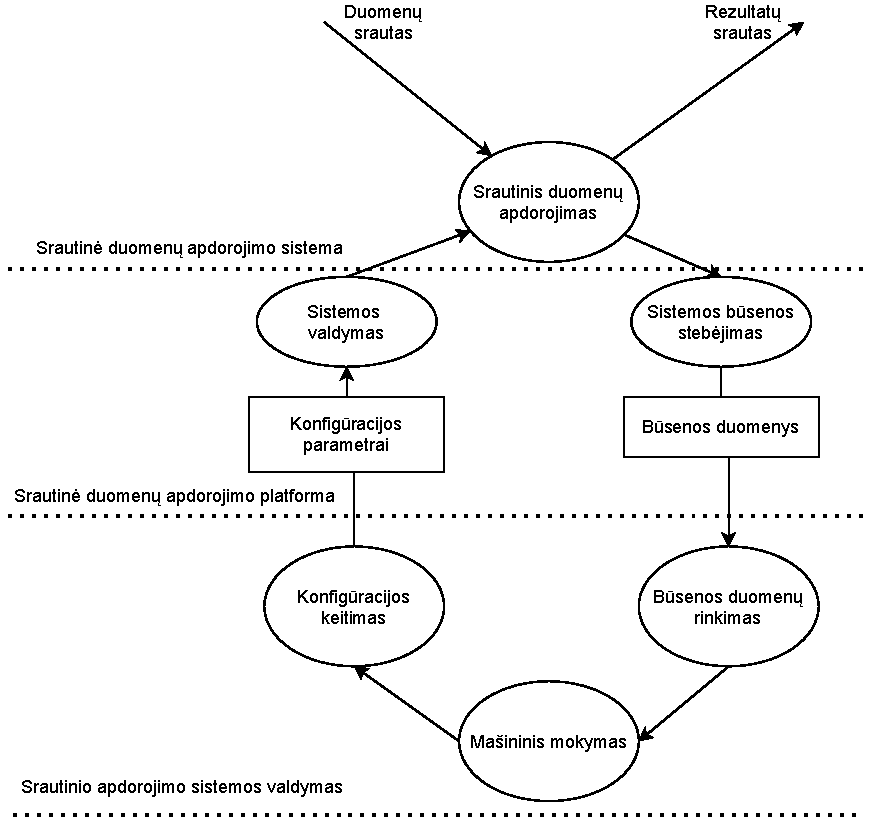
\includegraphics[width=15cm]{img/DataFlow.pdf}
    \caption{Srautinės apdorojimo sistemos modelis}
    \label{dataflow}
\end{figure} 
Srautinės duomenų apdorojimo sistemą sudaro šie elementai:
\begin{itemize}
    \item Duomenų srautas – duomenys patenkantys į srautinio apdorojimo sistemą nepertraukiamu srautu, iš anksto nežinomu greičiu ir nekontroliuojamu kiekiu.
    \item Srautinis duomenų apdorojimas – srautinio duomenų apdorojimo sistema, atliekanti skaičiavimus su duomenimis ateinančiais iš duomenų srauto. Tyrime naudojamos Heron srautinio apdorojimo sistemos pasižymi individualiais skaičiavimo komponentais, kurie skaičiuoja kiekvieną patenkantį duomenį ir yra sukurti užtikrinant lygiagretumą komponento lygyje.
    \item Rezultatų srautas – duomenys apdoroti srautinio duomenų apdorojimo sistemos ir perduoti iš paskutinio skaičiavimo komponento į kitas sistemas.
\end{itemize}
Srautinio apdorojimo sistemų platforma turi šiuos elementus:
\begin{itemize}
    \item Srautinį duomenų apdorojimą.
    \item Sistemos būsenos stebėjimą – srautinio apdorojimo platformos sistema renkanti srautinio apdorojimo sistemų veikimo metrikas ir šias metrikas atskleidžianti į išorę. Tyrime naudojama Heron platforma metrikas pateikia kiekvienam skaičiavimo komponentui individualiai per HTTP protokolą arba į naudotojo pateiktą metrikų surinkimo sistemą.
    \item Būsenos duomenys – tai metrikos vaizduojančios kiekvienos srautinio apdorojimo sistemos skaičiavimo komponentų  veikimo rodiklius, tokius kaip vėlinimas, pralaidumas, apkrovos ir t.t.
    \item Konfigūracijos parametrai – tai konfigūracijos rinkinys kurį apibrėžia srautinio apdorojimo platforma. Šie konfigūracijos parametrai nurodo srautinės apdorojimo sistemos veikimą ir taip pat gali apibrėžti parametrus skirtus individualiems skaičiavimo komponentams. Tyrime naudojama Heron platforma apibrėžia ir valdo visus srautinės apdorojimo sistemos konfigūracijos parametrus bei skaičiavimo komponentų lygiagretumo konfigūraciją.
    \item Sistemos valdymas – konfigūracijos parametrų pateikimas į srautinio apdorojimo platformą. Šie konfigūracijos parametrai nurodo srautinės apdorojimo sistemos ir jos skaičiavimo komponentų veikimą. Tyrime naudojama Heron platformą leidžia pateikti konfigūracijos failą per komandinę eilutę. Pateikus konfigūraciją platforma sustabdo srautinę apdorojimo sistemą, atnaujina jos konfigūraciją ir paleidžia sistemą iš naujo. Kai sistema sustabdoma, taip pat nustojama ir skaityti duomenis iš duomenų srauto, o paleidus sistemą duomenys skaitomi toliau.
\end{itemize}
Srautinio apdorojimo sistemos valdymo elementai susidaro iš:
\begin{itemize}
    \item Būsenos duomenų rinkimo – tai sistema renkanti duomenis apie srautinės apdorojimo sistemos būseną iš srautinės apdorojimo platformos. Ši sistema atsakinga už aktualių metrikų surinkimą, kurios naudojamos suformuoti vaizdą apie srautinio duomenų apdorojimo sistemos būseną.
    \item Mašininio mokymosi – sistema, kurį gauna srautinės apdorojimo sistemos būsenos duomenis ir pagal tai apskaičiuoja naujas konfigūracijos parametrų reikšmes. Tyrime naudojamas skatinamasis mokymasis, kuris bando gerinti sistemos būseną apskaičiuojant geriausią veiksmą konfigūracijos keitimui ir mokosi iš prieš tai atliktų veiksmų.
    \item Konfigūracijos keitimo – sistema priimanti atnaujintus konfigūracijos parametrus ir pateikianti juos į srautinio apdorojimo platformą. 
\end{itemize}

Visumoje \ref{dataflow} paveikslėlis apibrėžia duomenų judėjimą srautinio duomenų apdorojimo sistemos valdymo modelyje. Srautinio apdorojimo sistema yra pagrindinis elementas atsakingas už patį duomenų apdorojimą ir veikia nepriklausomai nuo kitų elementų modelyje. Srautinio apdorojimo platforma talpina ir palaiko srautinio apdorojimo sistemas, taip pat suteikia prieiga gauti informaciją apie srautinio apdorojimo sistemų būseną bei suteikia galimybę valdyti srautinio apdorojimo sistemas. Srautinio apdorojimo sistemų valdymo elementai atsakingi už srautinės apdorojimo sistemos konfigūracijos keitimą pagal surinktus būsenos duomenis.

\subsection{Keičiami konfigūracijos parametrai}

Norint koreguoti konfigūracijos parametrus reikia siųsti atnaujinimo komandą su atnaujinto konfigūracijos failo vieta į Heron komandinės eilutės įrankį (toliau Heron CLI). Pateikus konfigūracijos parametrus Heron platformą perkrauna srautinio apdorojimo sistemą su naujais parametrais. 
Vienas iš pagrindinių srautinės apdorojimo sistemos konfigūracijos parametrų – skaičiavimo komponentų lygiagretumas, kuris nurodo kiek paleidžiama tam tikro komponento instancijų. Taip pat tai yra vienintelis keičiamas konfigūracijos elementas, kuris priklauso nuo valdomos srautinio apdorojimo sistemos apibrėžimo.

Visi kiti konfigūravimo parametrai \cite{configDocument}, kurie keičiami balansavimo metu pateikti \ref{param–table} lentelėje:

\begin{longtable}{|p{0.59\linewidth}|p{0.41\linewidth}|}
    \caption{Keičiami konfigūracijos parametrai}
    \label{param–table}\\
    \hline
    \rowcolor[HTML]{C0C0C0} 
    Parametras                                              & Paaiškinimas                                                                                 \\ \hline
    \endfirsthead
    %
    \endhead
    %
    component–parallelism=[skaičiavimo komponento pavadinimas]            & Tam tikro skaičiavimo komponento lygiagretumas                                 \\ \hline
    heron.instance.tuning.expected.bolt.read.queue.size                   & Numatomas skaitomos eilės dydis Bolt tipo komponentuose                        \\ \hline
    heron.instance.tuning.expected.bolt.write.queue.size                  & Numatomas rašomos eilės dydis Bolt tipo komponentuose                          \\ \hline
    heron.instance.tuning.expected.spout.read.queue.size                  & Numatomas skaitomos eilės dydis Spout tipo komponentuose                       \\ \hline
    heron.instance.tuning.expected.spout.write.queue.size                 & Numatomas rašomos eilės dydis Spout tipo komponentuose                         \\ \hline
    heron.instance.set.data.tuple.capacity                                & Didžiausias kiekis kortežų sugrupuotu vienoje žinutėje                        \\ \hline
    heron.instance.emit.batch.time.ms                                     & Didžiausias laikas Spout tipo komponentui išsiųsti gautą kortežą               \\ \hline
    heron.instance.emit.batch.size.bytes                                  & Didžiausias partijos dydis Spout tipo komponentui išsiųsti gautą kortežą       \\ \hline
    heron.instance.execute.batch.time.ms                                  & Didžiausias laikas Bolt tipo komponentui apdoroti gautą kortežą                \\ \hline
    heron.instance.execute.batch.size.bytes                               & Didžiausias partijos dydis Bolt tipo komponentui apdoroti gautą kortežą        \\ \hline
    heron.instance.internal.bolt.read.queue.capacity                      & Skaitomos eilės dydis Bolt komponentams                                        \\ \hline
    heron.instance.internal.bolt.write.queue.capacity                     & Rašomos eilės dydis Bolt komponentams                                          \\ \hline
    heron.instance.internal.spout.read.queue.capacity                     & Skaitomos eilės dydis Spout komponentams                                       \\ \hline
    heron.instance.internal.spout.write.queue.capacity                    & Rašomos eilės dydis Spout komponentams                                         \\ \hline
    heron.api.config.topology\_container\_max\_ram\_hint                  & Daugiausiai operatyvios atminties kiekio konteineriui išskyrimo užuomina       \\ \hline
    heron.api.config.topology\_container\_max\_cpu\_hint                  & Daugiausiai procesoriaus pajėgumo konteineriui išskyrimo užuomina              \\ \hline
    heron.api.config.topology\_container\_max\_disk\_hint                 & Daugiausiai kietojo disko atminties kiekio konteineriui išskyrimo užuomina    \\ \hline
    heron.api.config.topology\_container\_padding\_percentage             & Užuominų galimą paklaidą                                                       \\ \hline
\end{longtable}

\subsection{Naudojamos metrikos}
Metrikos iš Heron srautinio apdorojimo sistemų gali būti pasiektos keliais skirtingais būdais: darant užklausą į Heron API, skaitant iš tekstinio failo, kurį pildo Heron platformą arba naudojant savo sukurtą metrikų skaitymo priedą, kuris pateikiamas į Heron platformą prieš ją paleidžiant. Visos metrikos yra saugomos srautinio apdorojimo sistemos kiekvienam skaičiavimo komponentui. 

\ref{metrics–table} lentelėje aprašytos metrikos yra standartinės visiems Heron srautinio apdorojimo sistemos komponentams ir grąžinamos iš Heron per Heron API \cite{heronTracker}. Šios metrikos perduodamos į mašininio mokymosi algoritmą.

\begin{longtable}{|p{0.5\linewidth}|p{0.4\linewidth}|}
    \caption{Naudojamos metrikos}
    \label{metrics–table}\\
    \hline
    \rowcolor[HTML]{C0C0C0} 
    Metriką                                  & Paaiškinimas            \\ \hline
    \endfirsthead
    %
    \endhead
    %
    \_\_emit–count (toliau išsiųstas kiekis)                           & Išsiųstų kortežų kiekis                    \\ \hline
    \_\_execute–count  (toliau apdorotas kiekis)                       & Apdorotų kortežų kiekis Bolt komponentuose \\ \hline
    \_\_execute–latency  (toliau vidutinis apdorojimo vėlinimas)       & Vidutinė trukmė Bolt komponentui apdoroti kortežą                                          \\ \hline
\end{longtable}

\subsection{Tikslo funkcija}

Srautinio apdorojimo sistemos valdymo tikslas – keičiant konfigūraciją, pasiekti didžiausią greitaveiką. Šiame tyrime greitaveika matuojama vėlinimu, todėl pasirinkta tikslo funkcija – tiesiogiai apskaičiuojamą pagal vėlinimą (\_\_execute–latency) ir duodamas teigiamas atlygis, jeigu pasiektas mažiausias vėlinimas, priešingu atveju neigiamas atlygis. 

\section{Balansavimo algoritmas}

\subsection{Srautinės architektūros sistemos konfigūracijos valdymo algoritmas}

Algoritmo tikslas – pagal esamą būseną ir esamą konfigūraciją apskaičiuoti naują konfigūraciją, kuri pagerintų srautinės apdorojimo sistemos greitaveiką. Algoritmo pagrindui yra pasirinkti skatinamojo mašininio mokymosi algoritmai REINFORCE, Deep Q Network ir Actor–Critic with Experience Replay.

Kad algoritmas galėtų apskaičiuoti naują konfigūraciją, jam reikalingi šie duomenys:
\begin{itemize}
    \item Dabartinė srautinio apdorojimo sistemos būsena - užklausos metų esantis komponentų lygiagretumas bei pasirinkta konfigūracija.
    \item Srautinio apdorojimo sistemos metrikos (\ref{metrics–table} lentelė) - atlygio apskaičiavimui.
    \item Srautinio apdorojimo sistemos pradinė konfigūracija (\ref{param–table–pract} lentelė).
    \item Veiksmų aibė kuriuos gali pasirinkti algoritmas.
\end{itemize}

Balansavimo algoritmas veikia ciklais visą srautinės apdorojimo sistemos veikimo laiką ir tarpas tarp ciklų turi būti pakankamai ilgas srautinio apdorojimo sistemai atsinaujinti su naujais konfigūracijos parametrais bei, kad surinktų duomenų kiekis būtų pakankamai svarūs pateikti mašininio mokymosi algoritmui. Balansavimo algoritmas, atlikęs skaičiavimus pasirenką veiksmą ir atlikęs jį laukia sekančio žingsnio. 

Balansavimui naudojami skatinamojo mašininio mokymosi algoritmai REINFORCE \cite{williams1992simple}, Deep Q network \cite{fan2020theoretical} ir Actor–Critic with Experience Replay \cite{wang2016sample} turi bendrus veikimo bruožus:
\begin{itemize}
    \item Jie yra laisvo nuo modelio (angl. model–free) tipo skatinamojo mokymosi algoritmai. Tai aktualu mūsų atveju kadangi balansavimo algoritmas turi galėti prisitaikyti prie kintančių duomenų kiekio ir greičio bei kintančios aplinkos.
    \item Jie yra be strategijos (angl. off–policy) tipo, tai reiškia, kad jie mokosi atliekant skirtingus veiksmus, nebūtinai tuos, kurie buvo pasirinkti pagal dabartinę strategiją.
\end{itemize} 

\subsection{Srautinio duomenų apdorojimo aplinkos apibrėžimas balansavimui}

Balansavimui atlikti reikalingas tikslus apibrėžimas srautinio apdorojimo aplinkos, šis apibrėžimas susidaro iš: galimų srautinio apdorojimo sistemos būsenų aibės, galimų veiksmų aibės ir funkcijų:
\begin{itemize}
    \item Inicializavimo funkcija - nustato pradinius sistemos parametrus, bei apibrėžia galimų veiksmų aibę ir aplinkos stebėjimo aibę.
    \item Žingsnio funkcija - kaip įeiti priima veiksmą, jį atlieką ir grąžina žingsnio rezultatus - būseną, atlygi ir t.t.
    \item Perrinkimo funkcija - grąžiną sistemą į pradinę būseną ir gražiną ją skatinamojo mokymosi algoritmui.
\end{itemize}

Kadangi pasirinkti algoritmai naudoja diskrečią veiksmų aibę, pasirinkta veiksmų aibė sudaryta iš srautinio apdorojimo komponentų lygiagretumo ir konfigūracijos rinkinio skaičiaus. Konfigūracijos parametrų rinkiniai sudaryti pagal \ref{param–table–pract} lentelėje pateiktas reikšmių aibes.

\begin{longtable}{|p{0.59\linewidth}|p{0.4\linewidth}|}
    \caption{Keičiamų konfigūracijos elementų aibė}
    \label{param–table–pract}\\
    \hline
    \rowcolor[HTML]{C0C0C0} 
    Parametras     & Natūraliųjų reikšmių aibė       \\ \hline
    \endfirsthead
    %
    \endhead
    %
    heron.instance.tuning.expected.bolt.read.queue.size       & \([2;20]\) \\ \hline
    heron.instance.tuning.expected.bolt.write.queue.size      & \([2;20]\) \\ \hline
    heron.instance.tuning.expected.spout.read.queue.size      & \([128;512]\) \\ \hline
    heron.instance.tuning.expected.spout.write.queue.size     & \([2;20]\) \\ \hline
    heron.instance.set.data.tuple.capacity                    & \([64;512]\) \\ \hline
    heron.instance.emit.batch.time.ms                         & \([8;128]\) \\ \hline
    heron.instance.emit.batch.size.bytes                      & \([8192;65536]\) \\ \hline
    heron.instance.execute.batch.time.ms                      & \([8;128]\) \\ \hline
    heron.instance.execute.batch.size.bytes                   & \([8192;65536]\) \\ \hline
    heron.instance.internal.bolt.read.queue.capacity          & \([64;512]\) \\ \hline
    heron.instance.internal.bolt.write.queue.capacity         & \([64;512]\) \\ \hline
    heron.instance.internal.spout.read.queue.capacity         & \([512;4096]\) \\ \hline
    heron.instance.internal.spout.write.queue.capacity        & \([64;512]\) \\ \hline
    heron.api.config.topology\_container\_max\_ram\_hint      & \([256;2048]\) \\ \hline
    heron.api.config.topology\_container\_max\_cpu\_hint      & \([20;80]\) \\ \hline
    heron.api.config.topology\_container\_max\_disk\_hint     & \([8192;65536]\) \\ \hline
    heron.api.config.topology\_container\_padding\_percentage & \([0;20]\) \\ \hline
\end{longtable}

Sudaryti 10 konfigūracijos rinkiniai išdalinus konfigūracijos elementus į lygias dalis pagal reikšmių aibę, siekiant, kad srautinės apdorojimo sistemos metrikos, atlikus vieną konfigūracijos pakeitimą, būtų žymus, kas leistų geriau pastebėti bei priduotų vertę atlikti konfigūracijos keitimą.

Sujungus konfigūracijos atnaujinimą ir komponentų lygiagretumo valdymo sudarytas galimų veiksmų rinkinys, kurio dydis yra lygus \(3 + (2 * \text{komponentų kiekis})\) ir kiekvieno veiksmo reikšmė pateikta \ref{action–space} paveikslėlyje.

\begin{longtable}{|p{0.1\linewidth}|p{0.6\linewidth}|p{0.1\linewidth}|p{0.1\linewidth}|}
    \caption{Galimų aplinkos veiksmų aibė}
    \label{action–space}\\
    \hline
    \rowcolor[HTML]{C0C0C0} 
    Veiksmo numeris                 & Veiksmas & Riba      \\ \hline
    \endfirsthead
    %
    \endhead
    %
    0                               & Nedaryti nieko & –  \\ \hline
    1                               & Pasirinkti konfigūracijos rinkinį, kurio numeris vienetų žemesnis & 0  \\ \hline
    2                               & Pasirinkti konfigūracijos rinkinį, kurio numeris vienetų aukštesnis & 10 \\ \hline
    1 + 2n                          & Atnaujinti n–tojo komponento konfigūracija, sumažinant jo lygiagretumą & 1 \\ \hline
    2 + 2n                          & Atnaujinti n–tojo komponento konfigūracija, padidinant jo lygiagretumą & 9 \\ \hline
\end{longtable}

Srautinio apdorojimo sistemos būsenos aibė – apibrėžiama kaip masyvas kuris susidaro iš srautinio apdorojimo komponentų lygiagretumo ir pasirinkto konfigūracijos rinkinio numerio. Pradinė būsena nustatyta, kad kiekvieno komponento lygiagretumo skaičius būtų 2, o pradinis konfigūracijos rinkinio numeris 5.

Skatinamojo mokymosi algoritmo veikimui reikalingas atlygis aplinkos apskaičiuojamas pagal formulę:
\[ Atlygis(n) =
\begin{cases}
    \text{min(Vėlinimas)} – \text{ Vėlinimas}_n  & \quad \text{Vėlinimas}_n \geq \text{min(Vėlinimas)}\\
    C – \text{ Vėlinimas}_n  & \quad \text{Vėlinimas}_n < \text{min(Vėlinimas)}
\end{cases}
\]
C – konstanta apskaičiuojama per pirmą paleidimą su pradinę konfigūracija, suapvalinus gautą vėlinimą. \newline
Srautinio apdorojimo sistemos balansavimo žingsnio funkcija susidaro iš:
\begin{itemize}
 \item Įeities – atliekamo veiksmo skaičiaus, kuris nurodo aplinkai kokį veiksmą ji turi įvykdyti.
 \item Išeities – atlikto veiksmo rezultatas, kuris susidaro iš:
 \begin{itemize}
    \item Būsenos – srautinio apdorojimo sistemos dabartinis komponentų lygiagretumas ir sistemos konfigūracija.
    \item Atlygio – apskaičiuoto naudojant metrikas gautas iš srautinio apdorojimo sistemos.
    \item Epizodo baigtumo rodiklio – nurodančio, ar aplinka baigė epizodą ir turi būti paleista iš naujo.
    \item Papildoma informacijos – naudojamos derinimo pagalbai.
 \end{itemize}
\end{itemize}

\subsection{Balansavimo algoritmo apmokymas}

Balansavimo algoritmo apmokymas yra atliekamas epizodais, kur vienas epizodas susidaro iš 25 žingsnių. Kiekvieno epizodo pradžioje srautinio apdorojimo sistemą perkraunama ir nustatoma su pradinėmis reikšmėmis. Visų algoritmų nagrinėjimui sistema buvo apmokoma nustatyta kiekį kartu ir po to naudojant apmokytą tinklą leidžiama atlikti sprendimus ant perkrautos srautinio apdorojimo sistemos. Pagrindinis srautinio apdorojimo sistemos balansavimo iššūkis - ilgas laiko tarpas tarp sistemos atnaujinimo. Tyrimui naudojama aplinka atlikusi pakeitimo veiksmą laukia 3 minutes, kas yra pakankamas laikas sistemai pasileisti ir pasiekti stabilią būseną. Dėl šios trukmės vienas epizodas trunka apie 1,5 valandos, kas yra pakankamai nemažas laiko tarpas žinant, kad norint pasiekti tikrai gerus rezultatus, gali tekti daryti apie 40 epizodų bei modifikuoti skatinamojo mokymosi algoritmą \cite{vaquero2018autotuning}. Šiame darbe pasirinkti nagrinėti trumpesnį apmokymo laikotarpį, bet skirtingų algoritmų ir su skirtingų kiekiu apmokytų epizodų siekiant patikrinti ar yra tendencija geresnio balansavimo priklausomai nuo algoritmo ir apmokymo kiekio. Kiekvienas algoritmo mokymai leidžiami iš naujo siekiant, kad rezultatai nebūtų įtakoti prieš tai atlikto mokymo dalies.

\section{Eksperimento tyrimo planas}

\subsection{Tyrimo tikslas}

Šio tyrimo tikslas – įvertinti siūlomo balansavimo modelio ir pasirinkto optimizavimo algoritmo validumą. Tam reikia atlikti bandymus su eksperimentine sistema naudojančia aprašyta optimizavimo algoritmą, su eksperimentine sistema naudojančia REINFORCE algoritmą ir su aplinka naudojančią standartinę konfigūracija be jokių pakeitimų. Gautus bandymo duomenis palyginti ir nustatyti, ar pasiūlytas sprendimas tinka srautinio apdorojimo sistemų balansavimui.

\subsection{Eksperimentinė sistema}

Eksperimentui atlikti naudojama lokali Heron aplinka ir papildomos posistemės skirtos duomenų generavimui, rezultatų rinkimui ir t.t. Pilna eksperimento sistema pavaizduota \ref{experiment} paveikslėlyje.

\begin{figure}[H]
    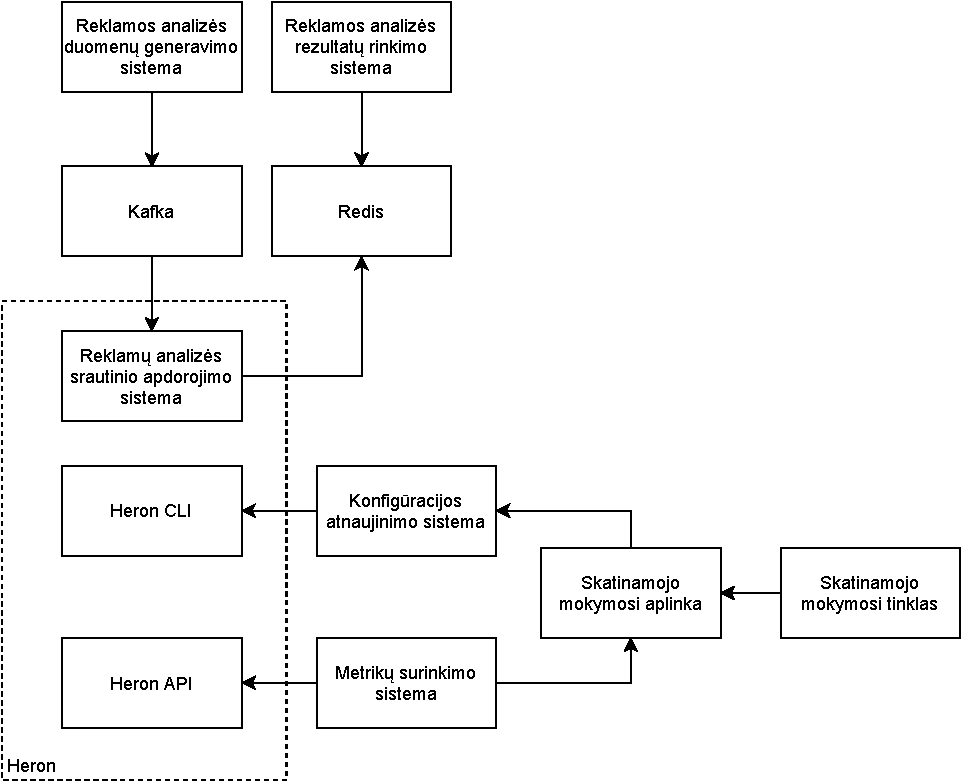
\includegraphics[width=14cm]{img/Experiment.pdf}
    \caption{Eksperimento sistemos architektūra}
    \label{experiment}
\end{figure} 

Sistemos, kurios naudojamos eksperimente:
\begin{enumerate}
    \item Skatinamojo mašininio mokymosi sistema. Kadangi atliekami bandymai su skirtingais skatinamojo mokymosi algoritmais, kiekvienam jų sukurta atskira sistema: 
    \begin{itemize}
        \item Skatinamojo mokymosi sistema naudojanti REINFORCE algoritmą, įgyvendinta naudojant tensorflow biblioteką ir oficialiai pateiktą dokumentaciją šio algoritmo įgyvendinimui. Taip pat šio algoritmo hiperparametrai sudėti pagal pateiktus \cite{vaquero2018autotuning} straipsnyje.
        \item Giliojo skatinamojo mokymosi sistema naudojanti Deep Q Network algoritmą, įgyvendinta naudojant tensorflow ir stable–baselines bibliotekas ir naudojant rekomenduojamus hiperparametrus.
        \item Giliojo skatinamojo mokymosi sistema naudojanti Actor–Critic with Experience Replay algoritmą, įgyvendinta naudojant tensorflow ir stable–baselines bibliotekas ir naudojant rekomenduojamus hiperparametrus.
    \end{itemize}
    \item Skatinamojo mokymosi aplinka – aprašanti srautinio apdorojimo sistemos būseną, veiksmų aibę ir konfigūracijos žingsnį, kuris atnaujina srautinio apdorojimo sistemą, surenką būsenos duomenis ir apskaičiuoja atlygio reikšmę. 
    \item Aplinkai reikalingos papildomos posistemės atlikti atnaujinimus ir surinkti duomenis:
    \begin{itemize}
        \item Metrikų surinkimo sistema parašyta Python kalba, naudojanti HTTP protokolą, būsenos duomenų surinkimui iš Heron API.
        \item Konfigūracijos atnaujinimo sistema parašyta su Python, skirta konfigūracijos atnaujinimui ir pateikimui į Heron sistemą per Heron CLI.
    \end{itemize}
    \item Reklamų srautinio apdorojimo sistema parašyta su JAVA, gaunanti duomenis iš Kafka žinučių eilės ir sauganti rezultatus Redis duomenų bazėje.
    \item Rezultatų apdorojimo sistema parašyta su Python, kuri surenka duomenis iš rezultatų failų, apdoroja juos ir grąžina skirtingų sprendimų diagramas.
    \item Reklamos analizės rezultatų rinkimo sistema parašyta su Clojure ir pateikta kartu su Reklamos analizės greitaveikos testu.
    \item Reklamos analizės duomenų generavimo sistema parašyta su Clojure ir pateikta kartu su Reklamos analizės greitaveikos testu.
\end{enumerate}

Kompiuterinės įrangos su kuria atliekamas eksperimentas parametrai:
\begin{itemize}
    \item Procesorius: Intel Core i7–5930k (6 branduoliai/12 gijų)
    \item Operatyvi atmintis: 64 GB (2666 MHz)
    \item Vaizdo plokštė: Nvidia GTX 1080Ti
    \item Operacinė sistema: Windows 10 Education
\end{itemize}

Kadangi Heron nepalaiko Windows sistemos visi tyrimai ir visos reikiamos posistemės leidžiamos naudojant Windows Subsystem Linux (toliau WSL) su Ubuntu 18.04. WSL yra suderinamumo sluoksnis naudojantis Linux branduolį per Hyper–V, kieno pagalba galima leisti programas skirtas Linux be emuliacijos neprarandant greitaveikos.

Pagrindinės programinės įrangos versijos:
\begin{itemize}
    \item Apache Heron: 0.20.3
    \item Kafka: 2.13
    \item Redis: 4.0.9
    \item Python: 3.6.9
    \item Java: 8
\end{itemize}
\subsection{Eksperimentų apimtis}

Eksperimentai atlikti su keturiais skirtingais sprendimais:
\begin{itemize}
    \item Srautinio apdorojimo sistemos veikimas su standartine konfigūracija.
    \item Srautinio apdorojimo sistemos veikimas balansuojant ją naudojant sukurtą eksperimentinį sprendimą pagal apibrėžtą balansavimo algoritmą naudojant:
    \begin{itemize}
        \item REINFORCE algoritmą skatinamojo mokymosi posistemėje.
        \item Deep Q Network algoritmą skatinamojo mokymosi posistemėje.
        \item Actor–Critic with Experience Replay algoritmą skatinamojo mokymosi posistemėje.
    \end{itemize}
\end{itemize}

Kiekvienas skatinamojo mokymosi sprendimas yra testuojamas su Reklamų analizės srautinio apdorojimo sistema.

Reklamų analizės sistema rezultatus talpina tekstini failą, kur kiekvienas įrašas yra vėlinimas milisekundėmis nuo paskutinio išsiųsto įrašo į žinučių eilę tam specifiniam kampanijos langui iki kol jis yra įrašomas į Redis duomenų bazę. Pasinaudojant šiais duomenimis, kiekvieną iteracija apskaičiuojamas vėlinimo vidurkis. 

Eksperimentai buvo atliekami su visais algoritmais apmokius juos 50 iteracijų, 100 iteracijų ir 250 iteracijų, tuo siekiant palyginti rezultatus tarp algoritmų ir bendra veikimą. Algoritmo efektyvumui patikrinti apmokytas modelis atlieka konfigūracijos keitimą 25 iteracijas ir matuojamas vėlinamas, kiekvieno po kiekvieno pakeitimo praėjus 3 minutėm, laikas kurio reikia srautinio apdorojimo sistemai pasileisti ir pasiekti pilną apkrovos stadiją.

\subsection{Eksperimento rezultatai}

Visuose grafikuose pateikiamos 25 iteracijos per kurias algoritmas nuo pradinės konfigūracijos atliko pakeitimus, kad pasiektų kuo mažesnį vėlinimą.
Kadangi srautinio apdorojimo sistemas paleistas Heron galima atnaujinti tik išjungus ir paleidus iš naujo, todėl kiekviena iteracija trunka virš trijų minučių, kas susidaro iš sistemos perkrovimo ir sistemos veikimo stabilizacijos.
\begin{figure}[H]
    \centering
    \begin{minipage}[b]{0.4\textwidth}
        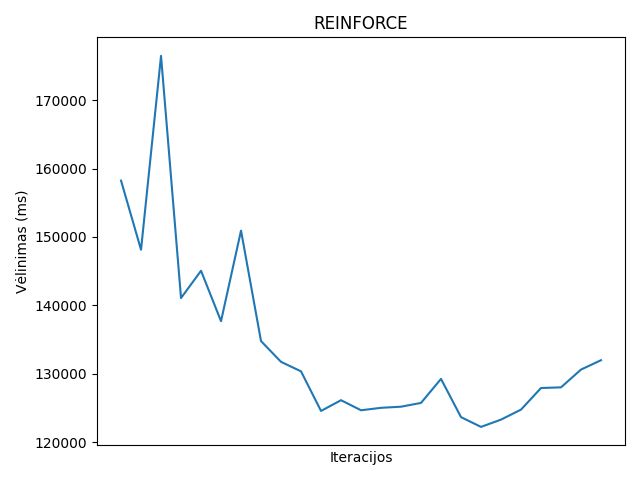
\includegraphics[width=\textwidth]{img/reinforce_50.png}
    \end{minipage}
    \hspace{100mm}
    \begin{minipage}[b]{0.4\textwidth}
        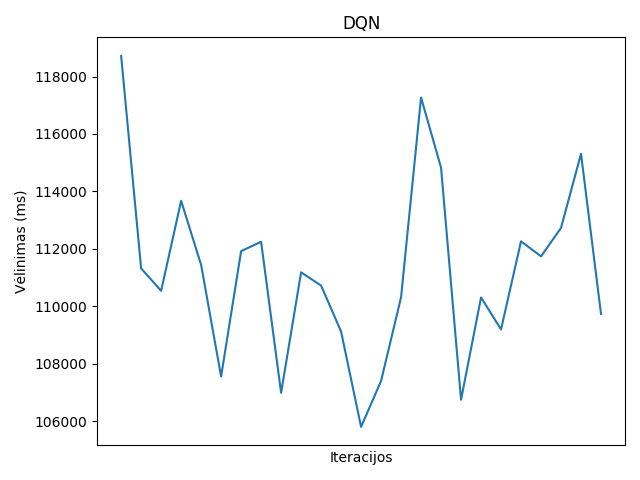
\includegraphics[width=\textwidth]{img/dqn_50.png}
    \end{minipage}
    \hspace{1mm}
    \begin{minipage}[b]{0.4\textwidth}
        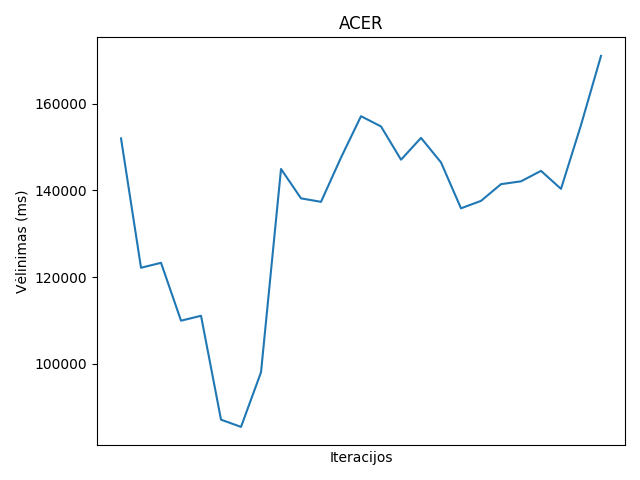
\includegraphics[width=\textwidth]{img/acer_50.png}
    \end{minipage}
    \caption{Skatinamųjų mokymosi algoritmų atliktas balansavimas po 50 mokymo iteracijų}
\end{figure}

\begin{figure}[H]
    \centering
    \begin{minipage}[b]{0.4\textwidth}
        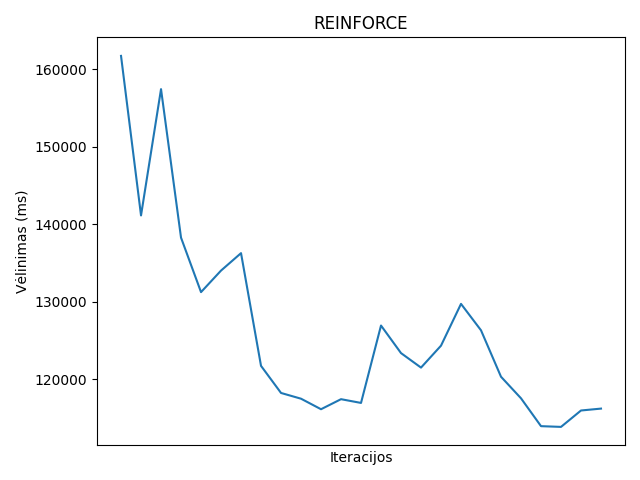
\includegraphics[width=\textwidth]{img/reinforce_100.png}
    \end{minipage}
    \hspace{100mm}
    \begin{minipage}[b]{0.4\textwidth}
        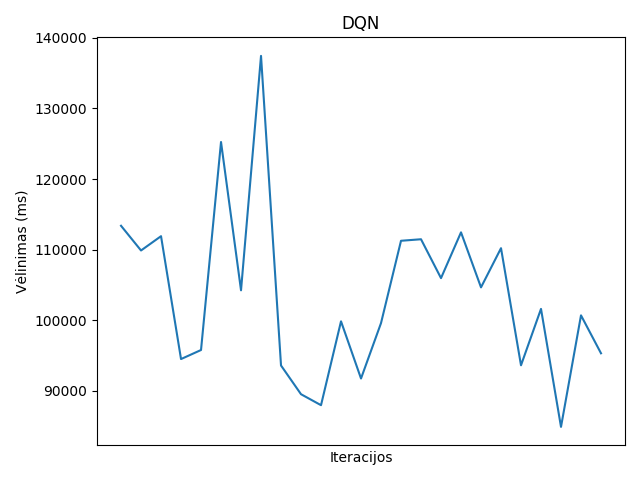
\includegraphics[width=\textwidth]{img/dqn_100.png}
    \end{minipage}
    \hspace{1mm}
    \begin{minipage}[b]{0.4\textwidth}
        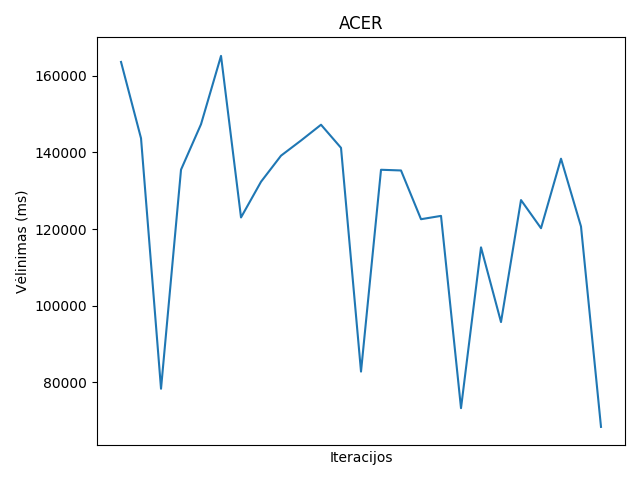
\includegraphics[width=\textwidth]{img/acer_100.png}
    \end{minipage}
    \caption{Skatinamųjų mokymosi algoritmų atliktas balansavimas po 100 mokymo iteracijų}
\end{figure}
\begin{figure}[H]
    \centering
    \begin{minipage}[b]{0.4\textwidth}
        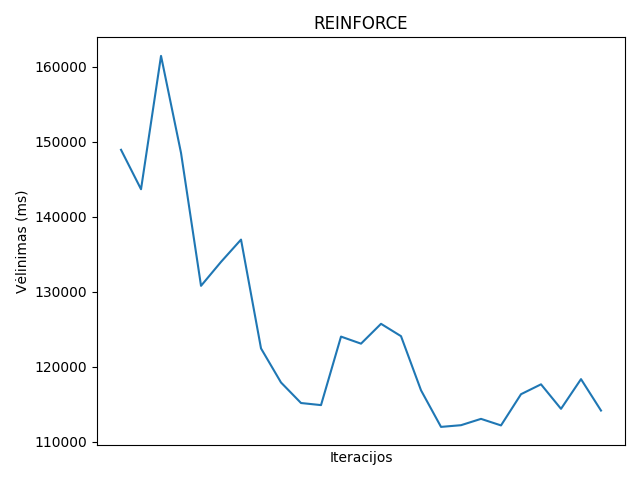
\includegraphics[width=\textwidth]{img/reinforce_250.png}
    \end{minipage}
    \hspace{100mm}
    \begin{minipage}[b]{0.4\textwidth}
        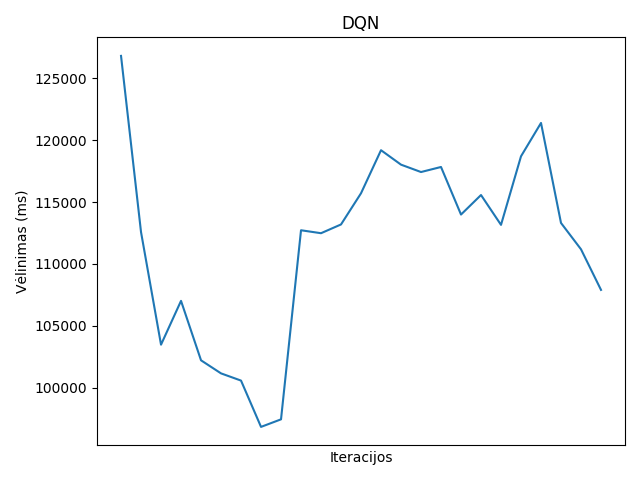
\includegraphics[width=\textwidth]{img/dqn_250.png}
    \end{minipage}
    \hspace{1mm}
    \begin{minipage}[b]{0.4\textwidth}
        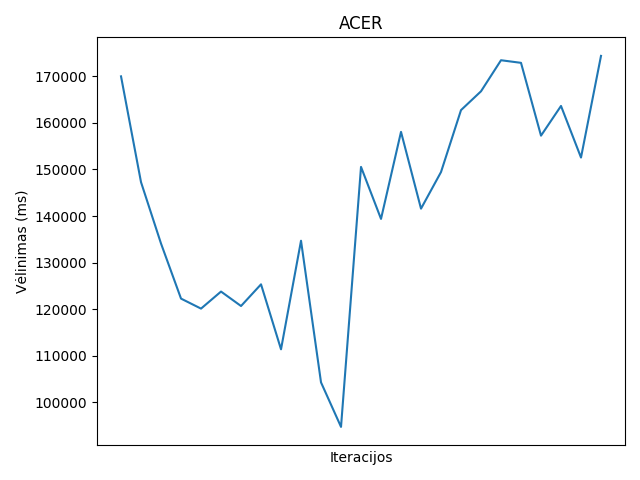
\includegraphics[width=\textwidth]{img/acer_250.png}
    \end{minipage}
    \caption{Skatinamųjų mokymosi algoritmų atliktas balansavimas po 250 mokymo iteracijų}
\end{figure}
      

\sectionnonum{Rezultatai ir išvados}
Rezultatai:
\begin{itemize}
    \item Sudarytas srautinės apdorojimo sistemos, valdomos skatinamuoju mokymusi, modelis.
    \item Apibrėžtas srautinio apdorojimo sistemos balansavimo algoritmas.
    \item Sukurta eksperimentinė sistemą ir atlikti eksperimentai su REINFORCE, Deep Q Network ir Actor–Critic with Experience Replay skatinamojo mokymosi algoritmais bei palyginti jų rezultatai.
\end{itemize}

Išvados:
Srautinio apdorojimo sistemas galima balansuoti naudojant skatinamąjį mokymąsi, tačiau tam reikia daug laiko apmokymui.
Giliojo skatinamojo mokymosi algoritmai pasirodo gerai, tačiau po daugiau apmokymo negu skatinamojo mokymosi algoritmai.
\printbibliography[heading=bibintoc] 

\end{document}
